\documentclass[12pt,a4paper]{article}
\synctex=1
\usepackage[utf8]{inputenc}
\usepackage[margin=1cm]{geometry}
\usepackage{graphicx}
%\usepackage{verbatim}
\usepackage{listings}
\usepackage{multicol}
\usepackage{libertine}
\usepackage{pgfornament}
\usepackage{eso-pic}
\usepackage{textcomp}
\usepackage{courier}
\usepackage[hangul]{kotex}
\linespread{1.3}

\title{
	\centering
	\pgfornament[width=12cm,color=teal]{84}\\
	\vspace{1cm}
	\fontsize{50}{50} \selectfont {시스템 S/W 실습6}\\
	\pgfornament[width=12cm,color=teal]{88}\\
	\vfill}
\author{
	\LARGE
	\begin{tabular}{rl}
		\hline
		학번 : & 2016110056\\ 
		학과 : & 불교학부 \\
		이름 : & 박승원\\
		날짜 : & \today\\
		\hline
	\end{tabular}\vspace{2cm}
	\\
	\includegraphics[width=0.5\textwidth]{/home/zezeon/Dropbox/Photos/logo.jpg}
}
\date{}


\begin{document}
\maketitle
\noindent
\lstset{columns=flexible, tabsize=4, frame=single, showstringspaces=false, breaklines=true, upquote=true}
\begin{enumerate}

\pagenumbering{gobble}
\lstset{language=C}
%\begin{multicols}{2}
\item 다음에 주어진 file 입출력을 위한 예제 프로그램을 참고하여 SIC srcfile을 assemble할 때 출력되는 OBJFILE을 입력해서 각 줄을 다음 중 한가지로 분리하여 tmpfile에 TAG, PROGNAME, ADDR, SIZE, CODES 등을 출력하는 프로그램을 작성하고 실습하시오. 
C Program compile 명령은 다음과 같다.

\vspace{1cm}
단, 입력파일 srcfile과 OBJFILE은 각자 준비하며, OBJFILE의 내용은 다음중 한가지의 형식으로 되어있다.

\$g++ -o test5 test5.c\\
\$./test6 srcfile \textgreater intfile


OBJFILE 형식:
TAG, PROGNAME, ADDR1, ADDR2\\
(Col.1: 'H', Col.2\~7: program name, Col.8-13:ADDR1, Col.14-19:ADDR2)\\
TAG,ADDR,LENGTH,CODES\\
(Col.1: 'T', Col.2-7:ADDR, Col.8-9:LENGTH,Col.10-60:CODES)\\
TAG,ADDR,OTHERS\\
(Col.1: 'M' 혹은 'E', Col.2-7:ADDR, Col.8-9:LENGTH, Col.10-60:OTHERS)

srcfile
\begin{lstlisting}
	htest 001000000018
	t001000090010060c1009000005
	e001000
\end{lstlisting}

test6.cc
\begin{lstlisting}
	#include<sstream>
	#include<string>
	#include<fstream>
	#include<iostream>
	#include<iomanip>
	using namespace std;
	
	int main(int c, char** v)
	{
		ifstream f(v[1]);
		char ch, TAG;
		string addr1, addr2, len;
		string s;
		f >> TAG >> s >> setw(6) >> addr1 >> setw(6) >> addr2;
		cout << "TAG : " << TAG << endl;
		cout << "PROGNAME : " << s << endl;
		cout << "ADDR1 : " << setw(6) << setfill('0') << hex << stoi(addr1, nullptr, 16) << endl;
		cout << "ADDR2 : " << setw(6) << setfill('0') << hex << stoi(addr2, nullptr, 16) << endl << endl;
	
		do {
			f >> TAG >> setw(6) >> addr1 >> setw(2) >> hex >> len >> s;
			cout << "TAG : " << TAG << endl;
			cout << "ADDR : " << setw(6) << setfill('0') << hex << stoi(addr1, 	nullptr, 16) << endl;
			cout << "LENGTH : " << len << endl;
			cout << "CODES : " << s << endl << endl;
		} while(TAG == 't');
		
		f >> TAG >> s;
		cout << "TAG : " << TAG << endl;
		cout << "OTHERS : " << s << endl;
	}
	
\end{lstlisting}

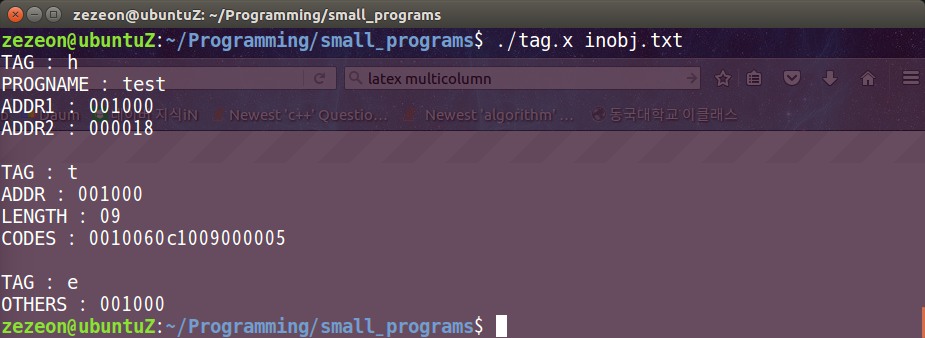
\includegraphics[width=\textwidth]{test6.png}
\end{enumerate}
{\Huge소감}
\indent
파일을 stdout으로 출력했다. 실행 코맨드를 test6 inobj.txt \textgreater out 으로 파이프를 이용하여 쉽게 파일로 보낼 수 있다.
\end{document}
